\begin{figure}[ht]
    \centering
    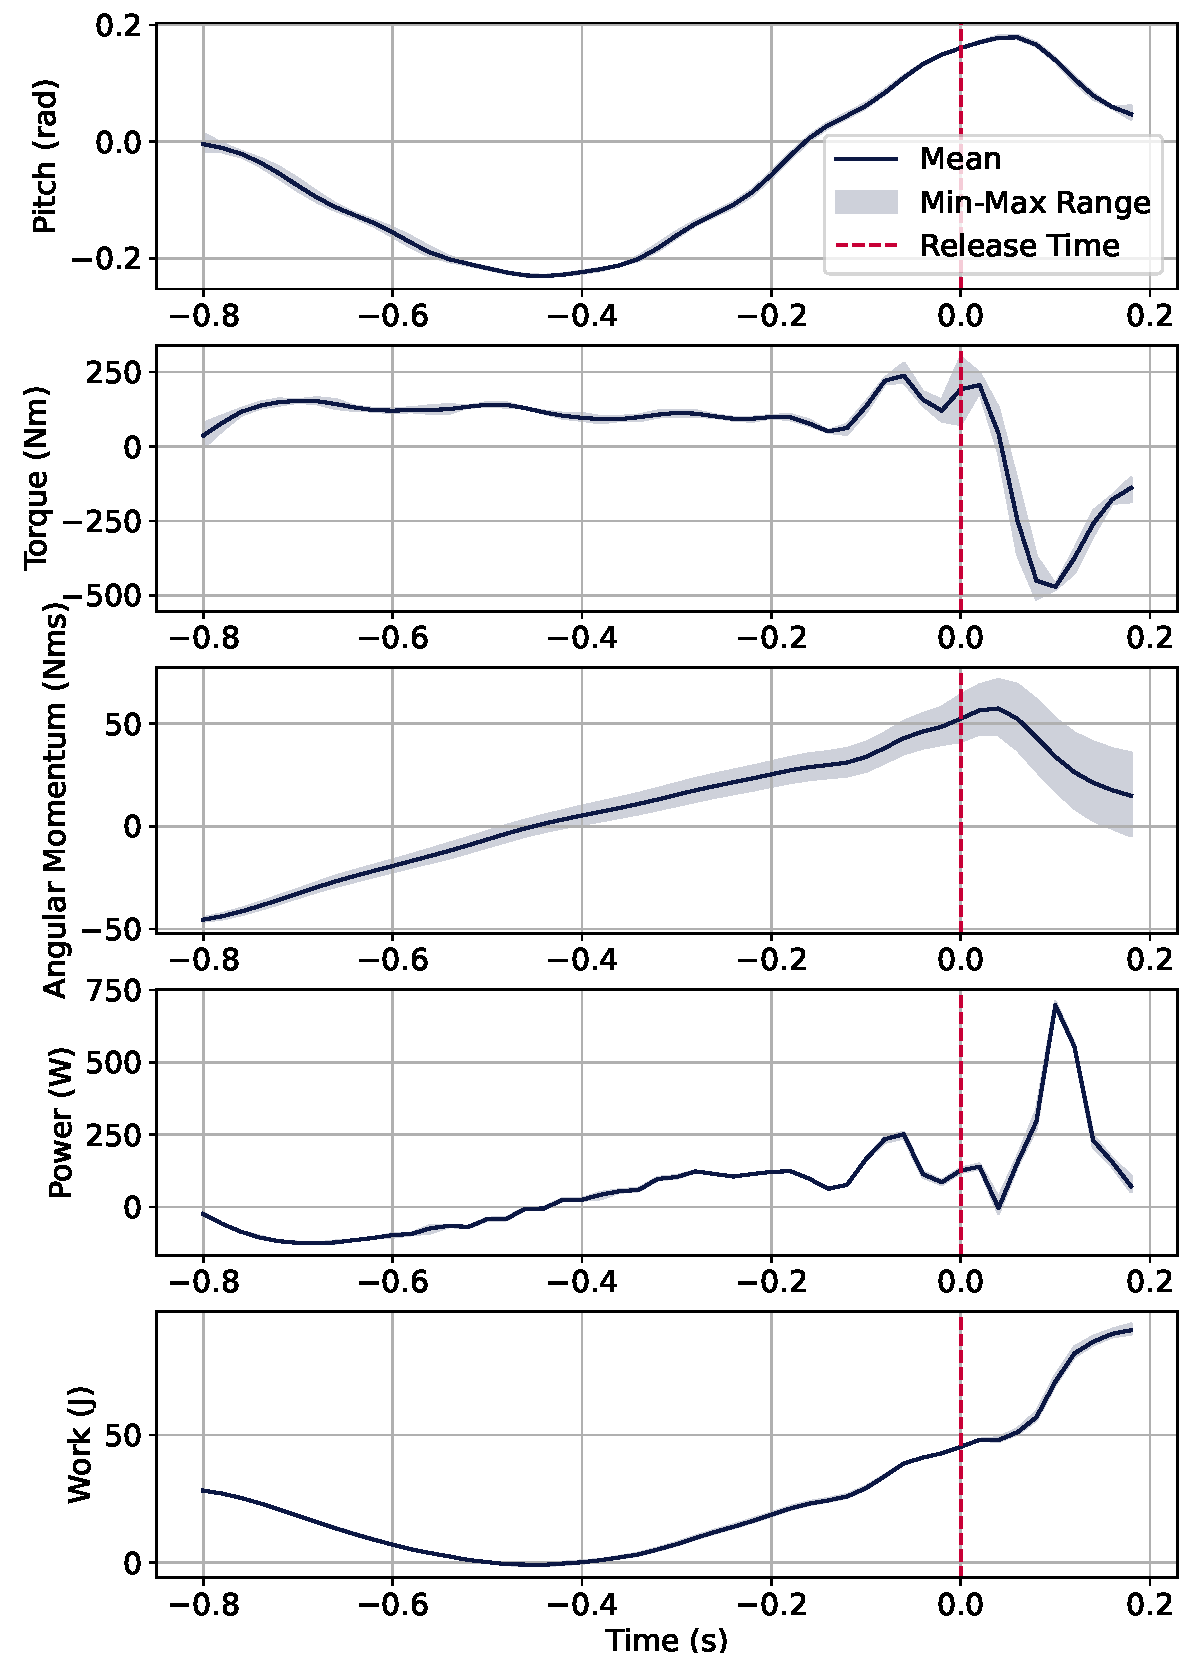
\includegraphics[width=0.48\textwidth]{figures/base_motion/base_motion1.pdf}
    \caption{\textbf{Base motion contributions to throws.} This figure illustrates the role of base motion in the throwing process by analyzing the base pitch angle, pitching torque, pitching angular momentum, power, and cumulative work. The angular momentum and cumulative work are calculated starting from the moment the base pitch rate turns positive. Data is derived from robot state estimation during hardware experiments for throws with a horizontal velocity of \unit[10]{m/s}.}
    \label{fig:base_motion}
    
    % \vspace{1.5cm}
\end{figure}
